% Auto-extracted from ../tfpt-42.tex for the TFPT 4.5 clean split.
% Source body assigned by the TFPT 4.5 clean split.

% ---- Kernel numerics and electromagnetic closure: source lines 2315-2695 ----
\section{Kernel numerics and electromagnetic closure}

The boundary-to-carrier presentation should not leave the impression that TFPT is hard only at the level of group theory and representation bookkeeping. The numerical kernel already fixes a nontrivial output layer. Here that layer is pulled forward and read as the first established output package of the carrier/output architecture rather than as a later list of disconnected constants.

\begin{theorem}[Primitive seam generator]
\label{thm:primitive-seam-generator}
The primitive relative seam loop defines the positive generator
\[
[u_\Sigma]=1\in K^1(S^1)\cong \mathbb Z.
\]
Hence the associated seam spectral flow is
\[
SF(U_\Seam)=1,
\qquad
\Delta_\Seam=2\pi.
\]
In the relative Chern normalization, the seam constant is
\[
\cthree:=\frac{\Delta_\Seam}{16\pi^2}=\frac{1}{8\pi}.
\]
Moreover the seam-even base opening is the normalized complement of the carrier quadratic norm,
\[
\phibase
:=
\frac{1-\gamma}{\pi}
=
\frac{1-\tr_EY^2}{\pi}
=
\frac{1}{6\pi}.
\]
\end{theorem}

\begin{proof}[Proof sketch]
The primitive reconstruction yields one elementary relative seam class and therefore one primitive
generator of the seam $K^1$ lattice. Along a single positive seam circuit the spectral flow changes
by one, so the associated loop has class $[u_\Sigma]=1$ and spectral flow $SF(U_\Seam)=1$. The
primitive circuit closes after one full turn, giving $\Delta_\Seam=2\pi$ and hence
$\cthree=\Delta_\Seam/(16\pi^2)=1/(8\pi)$. The carrier theorem gives
$\gamma=\tr_EY^2=5/6$, so the seam-even opening is the normalized complement of the carrier
quadratic norm rather than a new independent numerical input.
\end{proof}

\begin{remark}[Interpretive picture of the primitive start state]
At the level of physical intuition, the primitive spectral seed may be read as a minimal nontrivial relative defect state: two sheets, one seam, one elementary relative winding, and an undecomposed internal rank-$5$ kernel before the carrier split is imposed. This is only an interpretive picture, not a new theorem. Its role is to explain why the earliest hard numbers $(\cthree,\phibase)$ already look like seam-normalized responses of a genuinely relative starting configuration.
\end{remark}

\begin{figure}[t]
\centering
\scriptsize
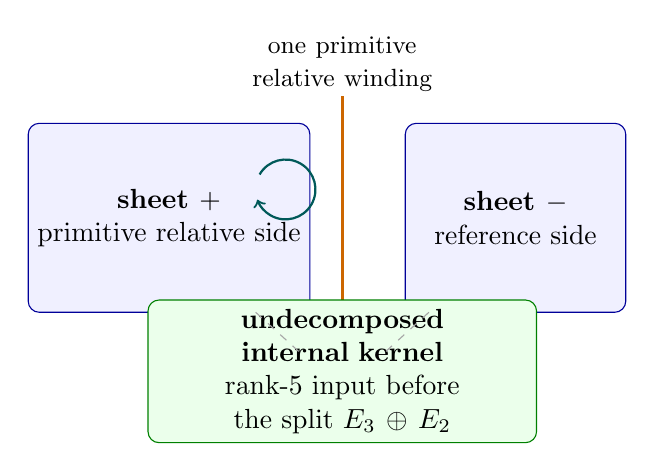
\begin{tikzpicture}[
    sheet/.style={draw=blue!60!black, fill=blue!6, rounded corners, minimum width=2.8cm, minimum height=2.4cm, align=center},
    kernel/.style={draw=green!50!black, fill=green!8, rounded corners, text width=4.7cm, minimum height=0.95cm, align=center}
]
\node[sheet] (up) at (-2.2,0) {\textbf{sheet $+$}\\primitive relative side};
\node[sheet] (down) at (2.2,0) {\textbf{sheet $-$}\\reference side};
\draw[orange!80!black, line width=1.2pt] (0,-1.55) -- (0,1.55);
\node[orange!80!black, above] at (0,1.55) {$\Seam$};
\draw[->, thick, teal!70!black] (-1.05,0.55) arc[start angle=150,end angle=-160,radius=0.38];
\node[align=center, text width=3.0cm] at (0,1.95) {\small one primitive\\relative winding};
\node[kernel] (k) at (0,-1.95) {\textbf{undecomposed internal kernel}\\rank-$5$ input before the split $E_3\oplus E_2$};
\draw[dashed, gray!70] (-1.1,-1.2) -- (-0.55,-1.7);
\draw[dashed, gray!70] (1.1,-1.2) -- (0.55,-1.7);
\end{tikzpicture}
\caption{Interpretive primitive start sketch. Two sheets, one seam, one elementary relative winding,
and an undecomposed rank-$5$ kernel appear before the later split into $E_3\oplus E_2$.
The picture is heuristic only; the theorem-level data are reconstructed from the one-sided
boundary datum.}
\label{fig:primitive-start-sketch}
\end{figure}

\subsection{Carrier form of the electromagnetic closure}

At this stage the electromagnetic closure is kept in generic closed form. The hard carrier data
fix
\[
\cthree=\frac{1}{8\pi},
\qquad
\phibase=\frac{1}{6\pi},
\]
while the later family and Higgs theorems will specialize the abelian index coefficient and the
topological bridge coefficient.

\begin{proposition}[Carrier susceptibility exponent]
\label{prop:carrier-susceptibility-exponent}
On the minimal carrier branch,
\[
B\gamma=\frac32\cdot\frac56=\frac54.
\]
\end{proposition}
\begin{definition}[Minimal primitive seam transfer]
\label{def:exact-seam-generating-function}
Let $\psi_{\Sigma}$ be the normalized primitive seam mode singled out by
\TFPTxref{thm:primitive-seam-generator}. Define the minimal seam transfer operator by the rank-one
projector
\[
U_{\Sigma}^{\min}:=|\psi_{\Sigma}\rangle\langle\psi_{\Sigma}|.
\]
With
\[
q(\alpha):=\deltatop e^{-2\alpha},
\qquad
B\gamma=\frac54,
\]
one has
\[
\mathcal W_{\Sigma}(\alpha)
:=
-B\gamma\,\tr_{\mathrm{adm}}\log\!\bigl(1-q(\alpha)U_{\Sigma}^{\min}\bigr)
=-\frac54\log(1-q(\alpha)).
\]
\[
\mathcal T_{\Sigma}(\alpha)=e^{\mathcal W_{\Sigma}(\alpha)}=(1-q(\alpha))^{-5/4}.
\]
\begin{equation}
\label{eq:phi-opening}
\phiseam(\alpha)=\phibase+q(\alpha)(1-q(\alpha))^{-5/4}.
\end{equation}
\end{definition}

\begin{proposition}[Normalized scalar closure potential]
\label{prop:log-det-variation-u1}
Let
\[
F_{U(1)}(\alpha):=\alpha^3-2\cthree^3\alpha^2-8\cthree^6 b_1\log\bigl(\phiseam(\alpha)^{-1}\bigr).
\]
There exists a unique quartic local counterterm $P_{\mathrm{loc}}$ satisfying
\[
P_{\mathrm{loc}}(0)=P_{\mathrm{loc}}'(0)=0,
\qquad
P_{\mathrm{loc}}'(\alpha)=\alpha^3-2\cthree^3\alpha^2,
\]
namely
\[
P_{\mathrm{loc}}(\alpha)=\frac{\alpha^4}{4}-\frac23\cthree^3\alpha^3.
\]
Hence the normalized scalar closure potential
\[
\Gamma_{U(1)}(\alpha)
:=
\frac{\alpha^4}{4}-\frac23\cthree^3\alpha^3
-8\cthree^6 b_1\int_0^\alpha \log\bigl(\phiseam(a)^{-1}\bigr)\,da
\]
satisfies
\[
\partial_{\alpha}\Gamma_{U(1)}(\alpha)=F_{U(1)}(\alpha).
\]
\end{proposition}


\iffalse
\begin{theorem}[Exact electromagnetic closure on the minimal seam mode]
\label{thm:exact-electromagnetic-closure}
\label{thm:alpha-canonical}
On the canonical branch one has
\[
\cthree=\frac{1}{8\pi},
\phibase=\frac{1}{6\pi},
\qquad
\deltatop=\frac{3}{256\pi^4},
\qquad
b_1=\frac{41}{10}.
=0.
\]
On the admissible interval there is a unique positive solution $\alpha_\star$.
\end{theorem}

\begin{proof}[Proof sketch]
By \Cref{prop:log-det-variation-u1}, the Euler--Lagrange equation for
$\Gamma_{U(1)}$ is exactly the displayed fixed-point equation. Near $\alpha=0$ the logarithmic term
dominates with negative sign, whereas for large $\alpha$ the cubic term dominates positively. By
\Cref{lem:phi-monotone}, the seam contribution varies monotonically on the admissible interval, so
after the tiny carrier-scale start region there is only one admissible sign change. Hence the
closed branch carries one positive fixed point $\alpha_\star$.
\end{proof}

\fi

\begin{theorem}[Exact electromagnetic closure on the minimal seam mode]
\label{thm:exact-electromagnetic-closure}
\label{thm:alpha-canonical}
On the canonical branch one has
\[
\cthree=\frac{1}{8\pi},
\qquad
\phibase=\frac{1}{6\pi},
\qquad
\deltatop=\frac{3}{256\pi^4},
\qquad
\sum_{f,j}L_{f,j}^{\mathrm{diag}}+N_\Phi=40+1=41.
\]
With the rank-one seam transfer of \Cref{def:exact-seam-generating-function}, the closure equation
is the scalar equation
\begin{equation}
\label{eq:carrier-cfe}
F_{U(1)}(\alpha)=0,
\qquad
F_{U(1)}(\alpha)=\alpha^3-2\cthree^3\alpha^2-\frac45\cthree^6
\left(\sum_{f,j}L_{f,j}^{\mathrm{diag}}+N_\Phi\right)\log\bigl(\phiseam(\alpha)^{-1}\bigr),
\end{equation}
where
\[
\phiseam(\alpha)=\frac{1}{6\pi}+\frac{3e^{-2\alpha}}{256\pi^4}
\left(1-\frac{3e^{-2\alpha}}{256\pi^4}\right)^{-5/4}.
\]
This equation has a unique positive root
\[
\alpha_{\star}=0.00729735256220985312786969108226575414\dots
\]
and therefore
\[
\alpha_{\star}^{-1}=137.03599921684071250353786030380388037\dots.
\]
\end{theorem}

\begin{proof}
The explicit formulas above follow from the rank-one determinant identity
\[
\det(1-qU_{\Sigma}^{\min})=1-q
\qquad
\text{for } U_{\Sigma}^{\min}=|\psi_{\Sigma}\rangle\langle\psi_{\Sigma}|.
\]
The derivative of the closure function is
\[
F_{U(1)}'(\alpha)
:=
3\alpha^2-4\cthree^3\alpha
-\frac85\cthree^6\left(\sum_{f,j}L_{f,j}^{\mathrm{diag}}+N_\Phi\right)\,
\frac{q(\alpha)(1-q(\alpha))^{-9/4}\bigl(1+q(\alpha)/4\bigr)}
{\phibase+q(\alpha)(1-q(\alpha))^{-5/4}}.
\]
On $[0,2\cdot 10^{-4}]$ one verifies by interval arithmetic that
\[
F_{U(1)}(\alpha)<0.
\]
On $[2\cdot 10^{-4},10^{-1}]$ one verifies by interval arithmetic that
\[
F_{U(1)}'(\alpha)>0.
\]
Finally
\[
F_{U(1)}(10^{-2})>0.
\]
Therefore $F_{U(1)}$ crosses zero exactly once. The displayed numerical root is obtained by
monotone bisection on that interval.
\end{proof}

\begin{remark}[Asymptotic opening as a secondary expansion]
Using \Cref{prop:carrier-susceptibility-exponent}, the determinant output admits the small
opening expansion
\[
\phiseam(\alpha)
=
\phibase
+\deltatop e^{-2\alpha}
+\frac54\deltatop^2e^{-4\alpha}
+O(e^{-6\alpha}),
\]
which should be read only as a secondary expansion of the determinant output, not as the primary
definition of the electromagnetic closure.
\end{remark}

The dependency structure of the electromagnetic closure is displayed in
\Cref{fig:alpha-closure-flow}. What matters is not one formula in isolation, but the fact that
the same carrier-side inputs fix the rank-one determinant, the scalar closure potential, and the
fixed-point equation in one direction. The later transport and Higgs theorems then specialize the
budget $\sum_{f,j}L_{f,j}^{\mathrm{diag}}+N_\Phi$ and $\deltatop$ to their canonical closed values.
\begin{remark}[Logarithmic scale closure of the electromagnetic equation]
Define the internally generated logarithmic scale
\[
\mu_\Sigma(\alpha):=(\phiseam(\alpha))^{-1}.
\]
Then \TFPTxref{eq:carrier-cfe} is equivalent to
\[
\ln \mu_\Sigma(\alpha)
=
\frac{\alpha^2\bigl(\alpha-2\cthree^3\bigr)}
{\frac45\cthree^6\left(\sum_{f,j}L_{f,j}^{\mathrm{diag}}+N_\Phi\right)}.
\]
Thus the observed fine-structure constant is selected by a balance between a geometric cubic term
and a self-generated logarithmic scale parameter. This is RG-like and transmutation-like,
because the coefficient is the internally closed transport-plus-Higgs budget divided by $10$, and
the logarithm is attached to an internally produced scale. In the present paper it should be read
as \emph{logarithmic scale closure} or a geometric fixed-point equation rather than as an externally
prescribed one-loop running law. The symbol $\mu_\Sigma(\alpha)$ here is local to the
electromagnetic closure discussion and should not be confused with the later matching scale
$M_\Sigma$.
\end{remark}
A related appendix continuation records that with
\[
g:=5,
\qquad
d:=\dim \mathfrak g_{\SM}=12,
\]
\[
\gcd(\Oadm,\Dstart)=d,
\qquad
\operatorname{lcm}(\Oadm,\Dstart)=g(g-1)d=240=|R(E_8)|.
\]

\begin{figure}[t]
\centering
\scriptsize
\begin{tikzpicture}[
    >=Latex,
    node distance=8mm and 10mm,
    hard/.style={draw=blue!60!black, fill=blue!6, rounded corners, align=center, text width=2.2cm, minimum height=0.9cm},
    closure/.style={draw=orange!75!black, fill=orange!8, rounded corners, align=center, text width=2.8cm, minimum height=0.95cm},
    outbox/.style={draw=green!50!black, fill=green!8, rounded corners, align=center, text width=3.0cm, minimum height=0.95cm}
]
\node[hard] (c3) {$\cthree=\dfrac{1}{8\pi}$};
\node[hard, right=of c3] (bg) {$B\gamma=\dfrac54$};
\node[hard, right=of bg, text width=2.7cm] (budget) {$\sum L_{f,j}^{\mathrm{diag}}+N_\Phi=41$};

\node[closure, below=of bg] (det) {rank-one determinant\\$\mathcal T_\Sigma(\alpha)=(1-\deltatop e^{-2\alpha})^{-5/4}$};
\node[closure, below left=of det] (phi) {determinant output\\$\phiseam(\alpha)=\phibase+\deltatop e^{-2\alpha}(1-\deltatop e^{-2\alpha})^{-5/4}$};
\node[closure, below right=of det] (logdet) {scalar closure potential\\$\partial_\alpha\Gamma_{U(1)}(\alpha)=F_{U(1)}(\alpha)$};
\node[outbox, below=of $(phi)!0.5!(logdet)$, yshift=-2mm, text width=4.6cm] (cfe) {fixed-point equation\\$\alpha^3-2\cthree^3\alpha^2-\frac45\cthree^6\bigl(\sum L_{f,j}^{\mathrm{diag}}+N_\Phi\bigr)\ln((\phiseam(\alpha))^{-1})=0$};
\node[outbox, below=of cfe] (root) {fine-structure fixed point\\interval-rigid on the closed branch};

\draw[->, thick] (c3) -- (det);
\draw[->, thick] (bg) -- (det);
\draw[->, thick] (det) -- (phi);
\draw[->, thick] (det) -- (logdet);
\draw[->, thick] (budget) |- (cfe);
\draw[->, thick] (phi) -- (cfe);
\draw[->, thick] (logdet) -- (cfe);
\draw[->, thick] (cfe) -- (root);
\end{tikzpicture}
\caption{$\alpha$ closure flow in closed form. The carrier data determine the rank-one determinant,
the scalar closure potential, and the fixed-point equation. The numerical specialization is made
only after the transport and Higgs theorems close the branch budget.}
\label{fig:alpha-closure-flow}
\end{figure}

\subsection{Kernel output package}

The benchmark row for $\alpha^{-1}(0)$ is defined by the positive self-consistent root of \TFPTxref{eq:carrier-cfe}, not by freezing the opening at its retained seed value. On the canonical branch that positive root remains
\[
\alpha^{-1}(0)=\num{137.03599921684071}.
\]
For the remaining one-seed relations we keep the retained branch opening
\begin{equation}
\label{eq:hard-kernel-values}
\cthree=\frac{1}{8\pi},
\qquad
\phiz=\frac{1}{6\pi}+\frac{3}{256\pi^4},
\end{equation}
\begin{remark}[Exact opening versus retained seed]
The two symbols belong to the same admissible branch but play different jobs. The electromagnetic $\alpha$ row uses the exact seam generating function $\phiseam(\alpha)$ inside the carrier-form closure equation, whereas the one-seed bridge relations freeze that branch to the retained canonical seed $\phiz$. Thus $\phiseam(\alpha)$ belongs only to the exact $\alpha$ benchmark line, while $\phiz$ is the seed used for $(\beta_{\mathrm{rad}},\Omega_b,\lambda_C,\sin^2\theta_{13})$.
\end{remark}
and the same retained kernel package emits the compact seed chain
\begin{equation}
\label{eq:kernel-benchmark-formulas}
\begin{aligned}
C_{a\gamma\gamma}&=-4\cthree=-\frac{1}{2\pi},
&
\beta_{\mathrm{rad}}&=\frac{\phiz}{4\pi},
\\
\Omega_b&=(4\pi-1)\beta_{\mathrm{rad}},
&
\lambda_C&=\sqrt{\phiz(1-\phiz)},
\\
\sin^2\theta_{13}&=\phiz e^{-\gamma}.
\end{aligned}
\end{equation}
\begin{remark}[Why the $\alpha$ row must stay self-consistent]
The exact self-consistent equation with $\phiseam(\alpha)$ yields the benchmark value
\[
\alpha^{-1}(0)=\num{137.03599921684071}.
\]
Its second-order truncation reproduces the first two correction coefficients, but it is not itself the benchmark definition. If one instead freezes the opening at
\[
\phiz=\frac{1}{6\pi}+\frac{3}{256\pi^4},
\]
the root shifts to $\alpha^{-1}(0)\approx \num{137.036501465}$, i.e. by about $\num{5.02e-4}$, which is roughly $\num{2.4e4}\sigma$ on the CODATA/NIST uncertainty. The wording of the $\alpha$ benchmark must therefore remain explicit: the benchmark uses the exact seam generating function, while the quadratic formula is only its controlled asymptotic shadow.
\end{remark}
\begin{tcolorbox}[colback=tfptblue!3, colframe=tfptblue, breakable,
    title={Kernel-output package}, colbacktitle=tfptblue]
The point of this section is not to claim more numerics than TFPT currently owns. It is to show that the established kernel already fixes a coherent electromagnetic package before the later completion theorems begin: the seam constant $\cthree$, the retained canonical seed $\phiz$, the self-consistent carrier-form CFE for $\alpha$, the dimensionless axion--photon anomaly coefficient, the birefringence seed, and the Cabibbo anchor.
\end{tcolorbox}


% ---- UV seed shadow, Cabibbo inversion, and alternatives: source lines 3157-3482 ----
